%% This is an example first chapter.  You should put chapter/appendix that you
%% write into a separate file, and add a line \include{yourfilename} to
%% main.tex, where `yourfilename.tex' is the name of the chapter/appendix file.
%% You can process specific files by typing their names in at the 
%% \files=
%% prompt when you run the file main.tex through LaTeX.
\chapter{Designing fecal microbiota transplant trials that account for differences in donor stool efficacy}

The contents of this chapter were submitted with
Scott W. Olesen$^*$, Thomas Gurry$^*$ (these authors contributed equally), and Eric J. Alm as authors.

The supplementary information is in Appendix B.
The supplementary tables are at the end of the chapter.

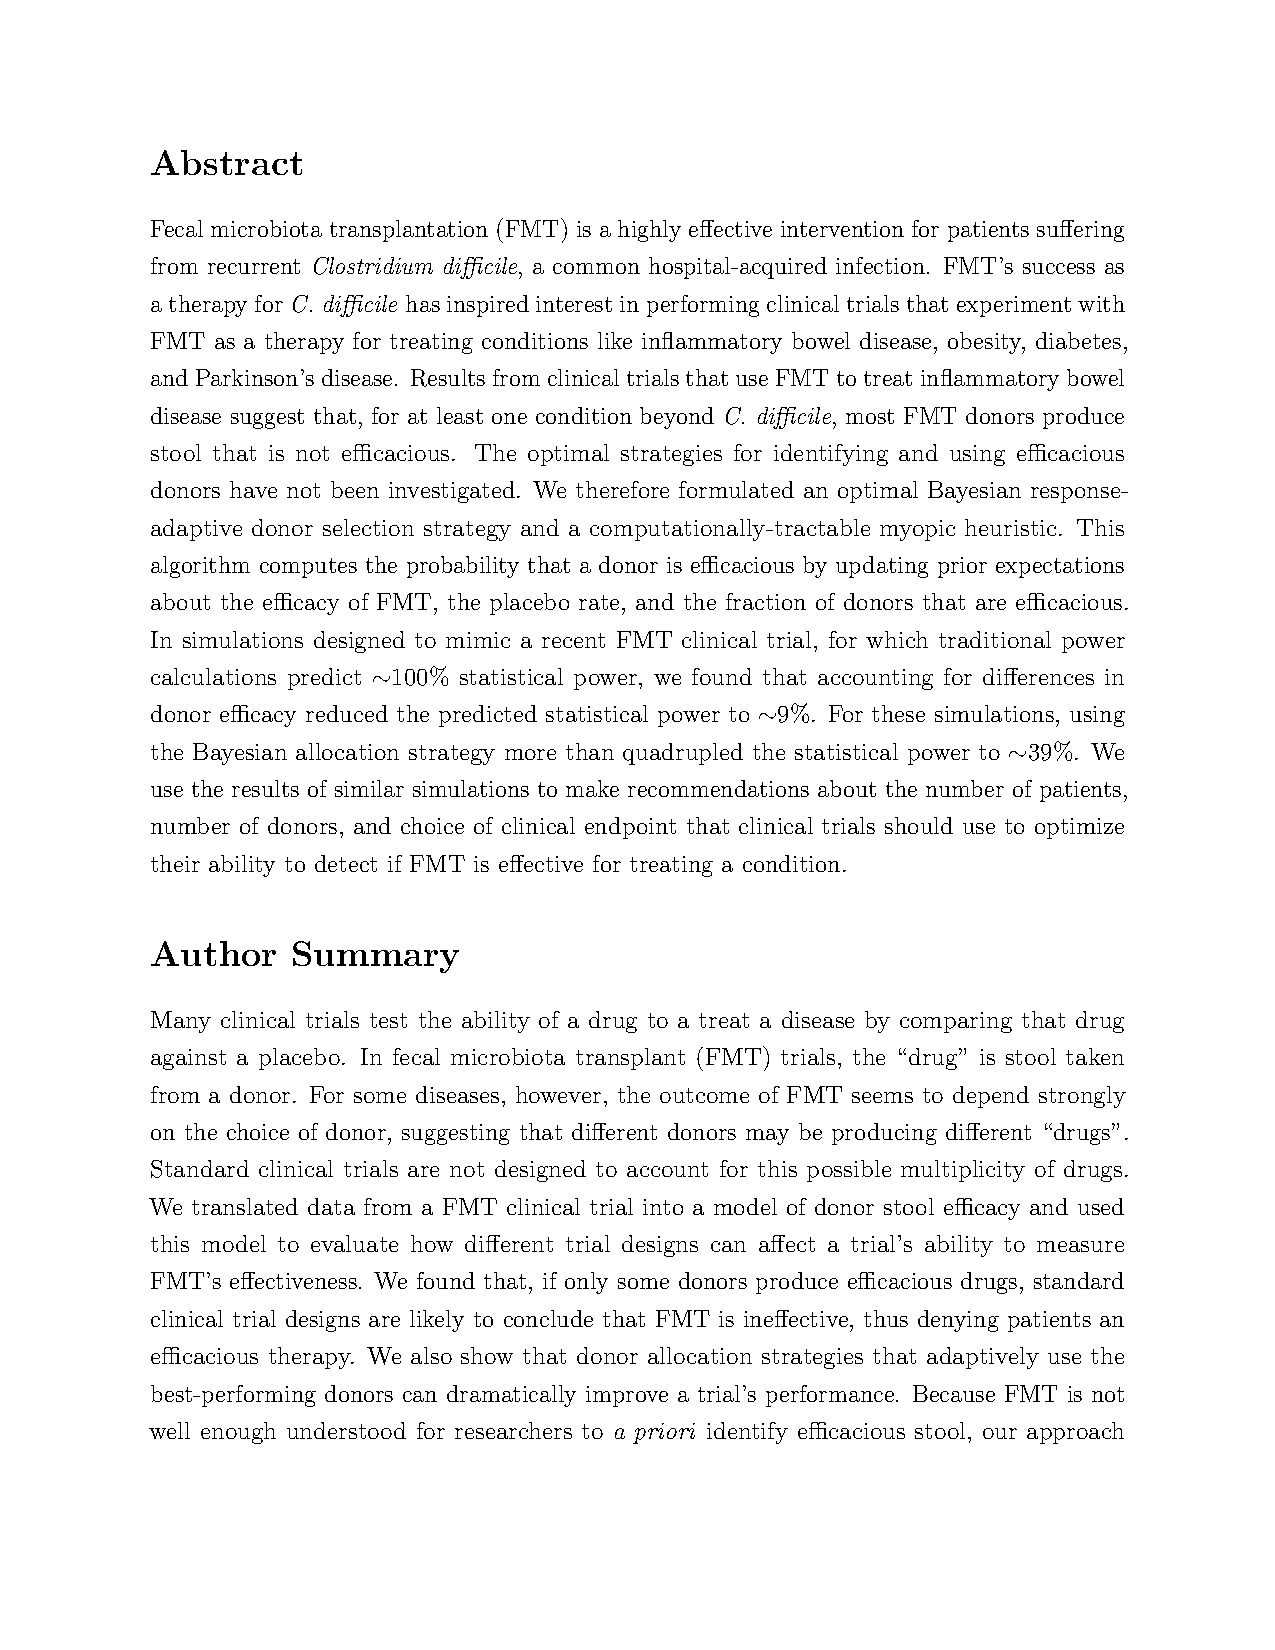
\includepdf[pages=-, pagecommand={\thispagestyle{plain}}, scale=0.95]{fmt/ms}
